% 
%jff-notes
%
\documentclass[11pt]{article}
\usepackage[pdftex]{graphicx}
\usepackage{amssymb}
\usepackage{latexsym}
%\usepackage{relsize}
\usepackage{textcomp}
%processed for 10 pt 
%\documentstyle[epsf,psfig]{article}
%\documentstyle[epsf]{article}
\oddsidemargin 0pt
\topmargin -0.0cm
\textwidth 6.2in
\textheight 8.5in
\baselineskip 18pt
%\renewcommand{\baselinestretch} {1.5}
\newenvironment{nitemize}
   {\begin{list}{\begin{math}\bullet\end{math}}%
      {\setlength{\leftmargin}{5mm}
       \setlength{\topsep}{1mm}
       \setlength{\parsep}{0in}
       \setlength{\itemsep}{.7mm}}}%
   {\end{list}}

\newcommand{\fract}[2]{\frac{\textstyle #1}{\textstyle #2}}
\newcommand{\trans}[3]{#1 \stackrel{#2}{\longrightarrow} #3}
\newcommand{\notrans}[3]{#1 \stackrel{#2}{\not\! \longrightarrow} #3}
\bibliographystyle{plain}
\begin{document}
\title{A simple NAVTEX plugin for SDRuno}
\author{
Jan van Katwijk\\
Lazy Chair Computing \\
The Netherlands\\
{\em J.vanKatwijk@gmail.com}}
%\date{}
\maketitle
%\baselineskip 22pt
\ \\
\ \\
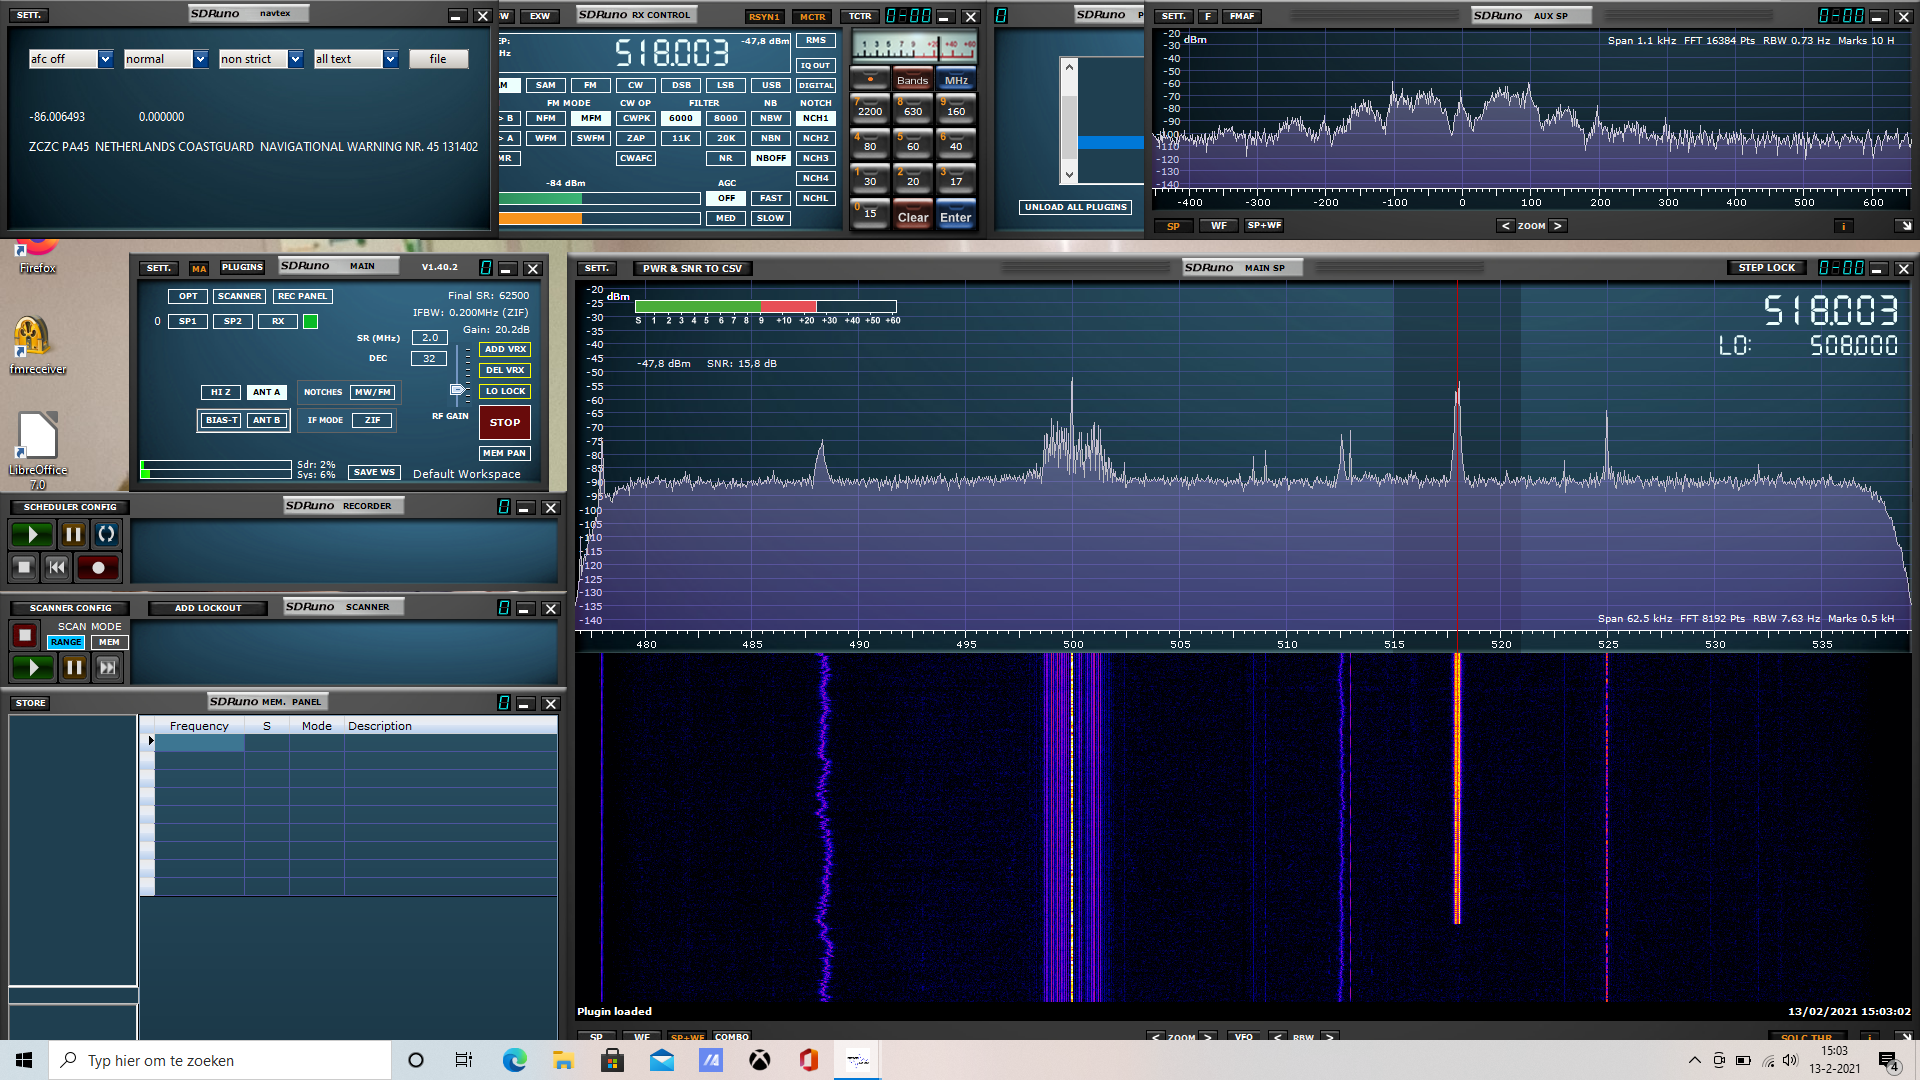
\includegraphics[width=140mm]{navtex-example.png}
\ \\
\section{Introduction}
NAVTEX (NAVigational TEleX) is a service for delivery of navigational and meteorological warnings and forecasts, as well as urgent maritime safety information (MSI) to ships. 

The transmissions are layered on top of SITOR collective B-mode. SITOR-B is a forward error correcting (FEC) broadcast that uses the CCIR 476 character set. NAVTEX messages are transmitted at 100 baud using FSK modulation with a frequency shift of 170 Hz.

The NavTex plugin can be used to receive and decode these messages,
the plugin will set tuning to 518KHz, the standard frequency for 
navtex messages (Another frequency for navtex messages is 490 KHz.)

\section{Settings}
navtex is a signal with a small footprint, the signal is transmitted as
an FSK signal, similar to RTTY, with a shift of  170 Hz and a baudrate of
100.

The decoder works similar to the rtty plugin, with an intermediate
samplerate of 12000 samples/second. Since the minimal samplerate for the
SDRplay family is 2000000, a lot of decimation has to be done.
\par
This implementation requires an input sample rate of 62500 samples/second,
this requires the setting of the mainwidget to a samplerate of 2000000,
and a decimation of 32, as shown in the picture

One should realize that the SDRuno spectrum display shows a band of 62.5
KHz, the advantage is that one sees a lot of signals, 
Fortunately, navtex messages are transmitted on fixed, predefined
frequencies.

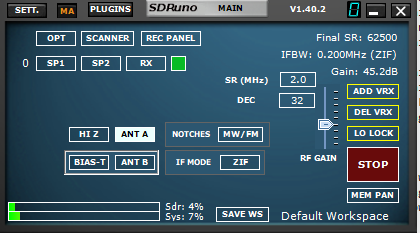
\includegraphics[width=100mm]{main-widget.png}

The plugin generates an audiotone of 800 Hz + the tuning offset,
In my experience a sound signal  is very helpful in precise tuning.
The sound is output with a rate of 48000, setting "AM" in the RX control window
will set this rate.

\section{Tuning}
As said, natex is a signal with a small footprint, however, it is
known in advance on which frequency the transmission will take place
and experience shows that tuning with the SDRplay family of devices
is pretty accurate.

Enlarging the auxiliary spectrum display, and zooming in as shown on the
picture shows the signal clearly.

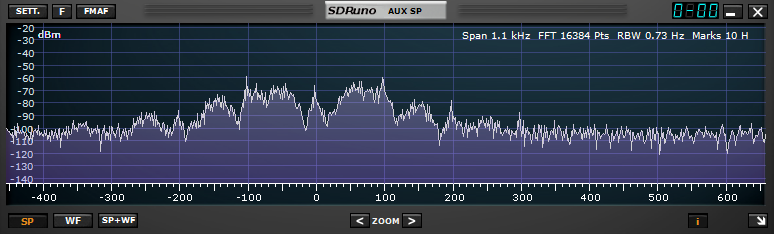
\includegraphics[width=100mm]{auxiliary-spectrum-display.png}

\section{The plugin}
The plugin widget  is shown in the picture

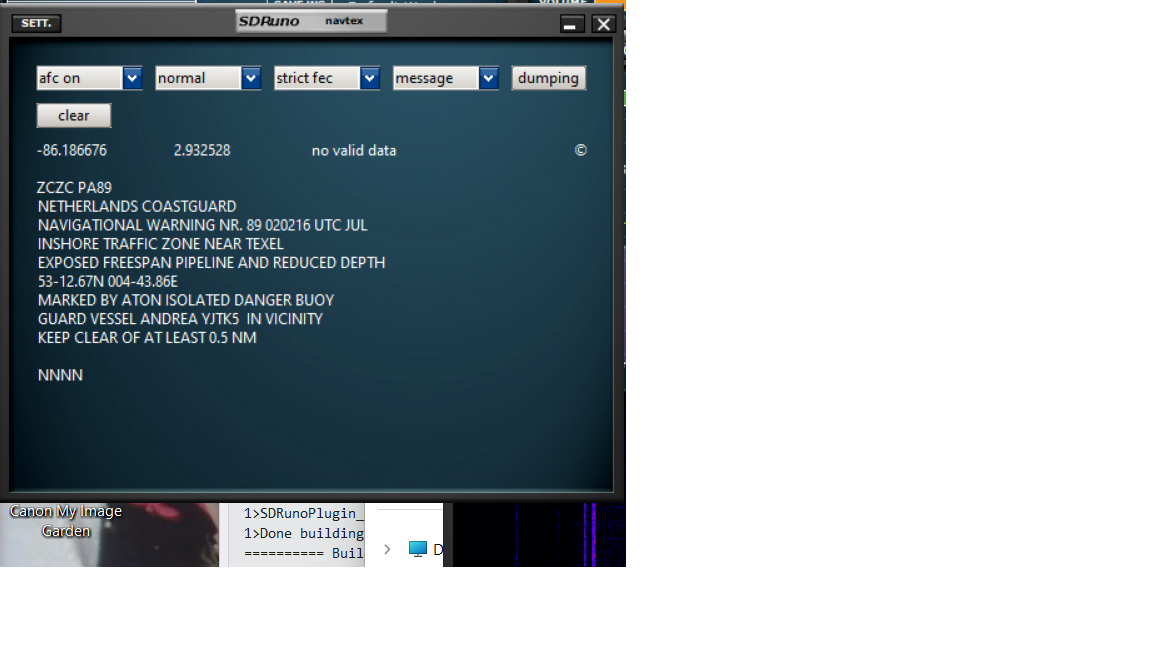
\includegraphics[width=100mm]{navtex-plugin-widget.png}

The widget has four control comoboxes and a button, from left to right
\begin{itemize}
\item the afc setting, choose between {\em afc on} and {\em afc off}. As usual,
with {\em afc on}  the software will try to correct the tuning. The
correction found is displayed in the number display on the right.
\item normal or reverse, choose switching the positions of the mark
and space elements in the signal;
\item the navtex signal has two levels of signal protection, the first one
is the Forward error correction. If {\em non strict} is chosen, data
will be output whether or not is passed the error check;
\item the second level is the format of the navtex message, if {\em all text}
is chosen all text is displayed, otherwise only messages passing the check
will be shown.
\item the file button, when touched shows a menu for file selection. All
output will - if a file is selected - be written as plain text in that
file.
Touching the button again (or unload the plugin) will close the file.
This feature is useful in combination with the selection of {\em message}
rather than {\em all text}. As known navtex messages are transmitted
only a few times per hour. Leaving the receiver tuned on 518 KHz, with
this plugin and this option selected, the radio can run for some time 
unattended, and later on received messages may be looked at.
\end{itemize}

\end{document}


